\chapter{Fundamentação Teórica}
\label{cap2}



\section{Jogos Eletrônicos}



O primeiro sistema de entretenimento interativo foi construído em 1947, utilizando como base de exibição um tubo de raios catódicos, criado por Thomas Goldsmith Jr. e Estle Ray Mann.
%
Essa criação foi patenteada em janeiro de 1948, datando então o início dos jogos eletrônicos~\cite{Adams2014Jan, patents1947Jan}.



O jogo eletrônico, ou entretenimento interativo, é uma atividade intelectual que integra um sistema de regras, na qual utiliza tal sistema a fim de definir seus objetivos ou pontuação por meio de um computador com o objetivo de dispertar alguma emoção ao jogador~\cite{video_game_technologies}.
%
Os jogos eletrônicos são aplicações convencionais, que executam sobre algum sistema operacional ou hardware apropriado a este fim.
%
O sistema operacional, hardware ou base de execução da aplicação gráfica define a sua plataforma, \textit{e.g.,} GNU/Linux, MS-Windows, Sony PS4, MS-XBox, web~\cite{adams_1208533}.



Inicialmente os jogos eram implementados de forma simples por conta da limitação das plataformas dos anos 80.
%
As implementações de jogos para videogames eram desenhadas diretamente para algum hardware proprietário, sem sistema operacional, por muitas vezes sem utilizar comunicação por rede ou memória de disco~\cite{adams_1208533}.
%
Já os jogos de computadores utilizando algum serviço online eram inviabilizados pelo custo de manutenção de tais serviços e pela baixa demanda de jogadores~\cite{adams_1208533}.
%
Na década de 80, o videogame Atari foi uma plataforma popular, vendendo 30.000 unidades em seu lançamento contra apenas 2.000 unidades do seu concorrente Intellivision~\cite{atari_age}. A sua especificação era:



O crescente recurso computacional disponível em computadores pessoais e videogames após os anos 90 permitiu que desenvolvedores criassem novos estilos de jogos que utilizavam de hardware mais especificado~\cite{adams_1208533}.
%
Dentre esses hardwares, iniciou-se o uso da rede de computadores para prover a interação entre jogadores de máquinas distintas~\cite{statisita_consumo_rede}.
%
Jogos como EA Habitat\footnote{EA Habitat: \url{http://www.mobygames.com/game/c64/habitat/credits}}, CipSoft Tibia\footnote{Tibia: \url{http://www.tibia.com/}} e Jajex Runescape\footnote{Jajex Runescape: \url{https://www.runescape.com}} começam a utilizar, como requisito obrigatório do jogo, a conexão com a Internet.
%
Tais jogos popularizaram trazendo uma inovação em seu quesito de jogabilidade e desafio proposto, criando uma nova subcategoria.



\subsection{Árvore de gêneros de jogos eletrônicos}



A classificação por gênero é uma ferramenta tradicional para auxiliar a fácil identificação de características de alguma literatura, arte e outras mídias.
%
Dentro de jogos eletrônicos, o gênero permite que jogadores comprem jogos com características próximas conforme o seu gosto\cite{Clarke2015}.



Um gênero de jogo eletrônico é uma categoria específica para agrupar estilos de jogabilidade parecidos.
%
Porém, gêneros não definem definitivamente o conteúdo expresso em algum título, mas sim um desafio comum presente no título analisado~\cite{adams_1208533, video_game_technologies}.
%
Cada gênero de jogo contém várias variações, para uma melhor classificação.
%
A árvore pode ser visualizada pelo diagrama na Figura \ref{fig:generos}.
%
O contexto breve de cada gênero é:




\begin{itemize}
  \item Estratégia: Jogos de estratégia são focados em uma jogabilidade que exija habilidades de raciocínio e/ou gerenciamento de recurso. Neste gênero, o jogador tem uma boa visualização do mundo, controlando indiretamente as suas tropas disponíveis~\cite{rollings2003andrew}. É comum encontrar jogos que disponibilizam algum modo de competição entre jogadores em uma rede local ou via Internet~\cite{adams_1208533}.
    \begin{itemize}
      \item \ac{rts}: Esse utiliza as características de um jogo de estratégia, porém esse subgênero indica que as jogadas dos jogadores não são atômicas~\cite{adams_1208533}.
    \end{itemize}
  \item Jogos Massivos: Esse gênero de jogo preza pela interação com outros jogadores em um mundo compartilhado~\cite{adams_1208533}. SecondLife\footnote{SecondLife: \url{https://www.secondlife.com/}} é um jogo focado na interação social, com artifícios de comércio e relacionamentos em um mundo fictício criado pela comunidade~\cite{tecmundo_secondlife}.
    \begin{itemize}
      \item \ac{moba}: Este gênero coloca um número fixo de jogadores separados em dois times, no qual o time com maior estratégia de posicionamento e gerenciamento de recursos em equipe ganha a partida. Jogos \ac{moba} perdem algumas características breves do gênero \ac{rpg}, deixando de lado a interpretação e contextualização de um mundo, fixando-se somente em um comate estratégico e momentânio (distribuído em partidas átomas) entre as equipes, carregando consigo somente as características de comércio e comunidade dos jogos \ac{mmo}~\cite{adams_1208533}. Tal subgênero é popularmente conhecido pelos títulos Blizzard Dota 2\footnote{Blizzard Dota 2: \url{http://br.dota2.com/}} e Riot League of Legends\footnote{Riot League of Legends: \url{https://br.leagueoflegends.com/pt/}}. O jogo League of Legends obteve 100 milhões de usuários ativos em 2016~\cite{lol_statista}, além de ter um torneio nacional e mundial~\cite{lol_sportv}.
      \item \ac{mmorpg}: Esse gênero herda características dos gêneros ação e aventura, \ac{rpg}, e \ac{mmo} diretamente. Nesse gênero, o jogo permite interações em um mundo na qual outros jogadores também estão jogando, permitindo a interação entre outros jogadores (herdado dos jogos \ac{mmo}), com o mundo (herdado dos jogos de ação e aventura), e com objetivos guiados por \ac{npcs} (herdados de jogos \ac{rpg})~\cite{adams_1208533}. Um título popular para esse gênero é o jogo Word of WarCraft\footnote{Word of WarCraft: \url{https://worldofwarcraft.com/pt-br/}}. Esse gênero será melhor abordado na Seção \ref{sec:mmorpg}.
    \end{itemize}
  \item Aventura: Este jogo é caracterizado por desafios envolvendo ações com diversos \ac{npcs} ou com o ambiente para solucionar desafios~\cite{adams_1208533}.
    \begin{itemize}
      \item Ação e Aventura: Esse gênero herda características da categoria de Ação e Aventura. O jogador é imerso em um mundo para iteragir com o ambiente e com \ac{npcs}, além de se preocupar com a movimentação no cenário~\cite{adams_1208533}. Um título popularmente conhecido desse gênero é a série de jogos nomeada Nintendo The Legend of Zelda\footnote{Nintendo The Legend of Zelda: \url{https://www.zelda.com/}}.
    \end{itemize}
  \item Simulação: Esse gênero de jogos são desenhados sobre aspéctos reais ou fictícios da realidade. Temas comums nesse gênero são jogos de construção e gerenciamento, animais de estimação, vida social e simulação de veículos~\cite{adams_1208533}.
    \begin{itemize}
      \item Esportes: Esse sub-gênero da simulação trata somente da simulação de esportes, nos quais o(s) time(s) podem ser controlados tanto por uma inteligência artificial quanto por jogadores online~\cite{adams_1208533}. O jogo FIFA\footnote{FIFA: \url{https://www.easports.com/br/fifa}} é um título popular nesse segmento.
    \end{itemize}
  \item Ação: Essa categoria de jogos preza pela habilidade de coordenação motora e reflexos do jogador, para tomar uma atitude a fim de passar seus objetivos no cenário. Nesse gênero os objetivos são passar por uma série de desafios que incluam movimentação e posicionamento de outros objetos no cenário~\cite{adams_1208533}.
    \begin{itemize}
      \item Jogos de Tiro: Em jogos de tiro, o jogador usa um número finito de armas para executar ações a distância. O posicionamento, movimentação estratégia e mira são fatores de desafio ao jogador nesse gênero~\cite{adams_1208533}.
        \begin{itemize}
          \item \ac{fps}: Nesse subgênero, o jogo utiliza o método de gravação conhecido como \ac{pov}. Nesse método, o modo de exibição do mundo é dado como a visão de um personagem do jogo, na qual o personagem não tem visão de sí próprio se não por reflexos~\cite{video_game_technologies, adams_1208533}.
          \item \ac{tps}: Diferente dos jogos \ac{fps}, os jogos \ac{tps} utilizam cameras soltas no cenário no qual o jogador é visível na cena exibida~\cite{video_game_technologies, adams_1208533}.
        \end{itemize}
    \end{itemize}
  \item Jogos sérios: Esse gênero de jogo tem como objetivo transmitir um conteúdo educacional~\cite{video_game_technologies}. O jogo Sherlock Dengue 8~\cite{sherlock_dengue} é um título desenvolvido com o objetivo de conscientizar os problemas e a prevenção da Dengue no Brasil.
\end{itemize}



\begin{figure}[htb!]
\caption{Árvore de gêneros simplificada.}
\label{fig:generos}
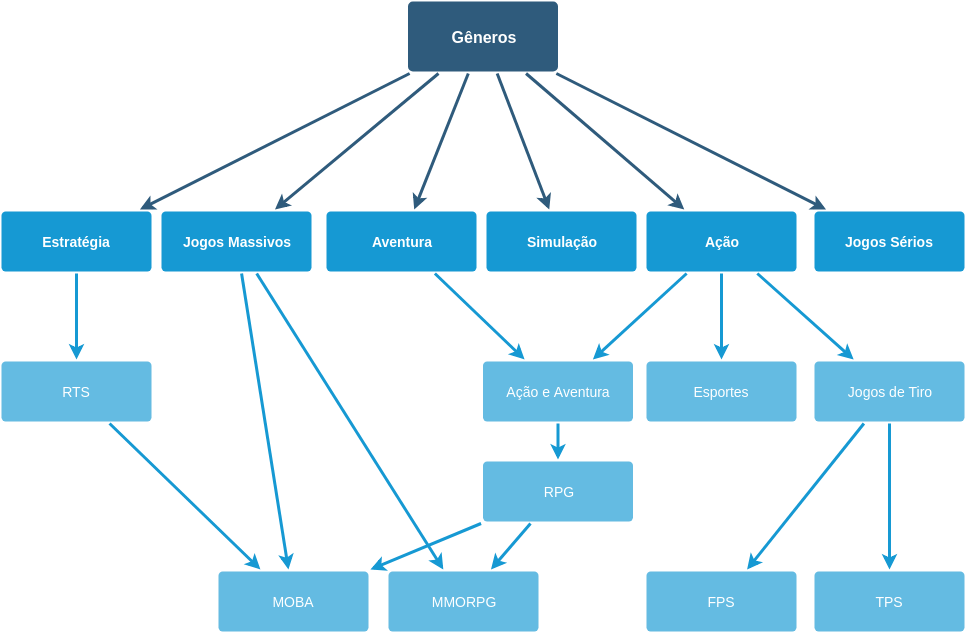
\includegraphics[height=9cm]{img/cap2/generos.png}
\centering

Adaptado de:~\cite{adams_1208533}
\end{figure}



O gênero abordado no atual documento refere-se à \ac{mmorpg}. O desenvolvimento desse gênero segue determinados padrões, tais como a necessidade de um serviço e um cliente (definidos na Seção \ref{sec:mmorpg}), problemas comuns com a indisponibilidade ou baixo desempenho do serviço e o custo de manutenção de tais serviços.



\section{Jogos Massivos}
\label{sec:mmorpg}



Jogos \ac{mmorpg} são utilizados como negócio viável e lucrativo, sendo que experiência de jogabilidade na qual o usuário final será submitido é um fator crítico para o sucesso.
%
O mercado de jogos \ac{mmorpg} vem crescendo desde 2012~\cite{new_york_times}, sendo no ano de 2016 um dos mais lucrativos~\cite{statista_2016}.
%
A sua projeção para 2018 é que sejam arrecadados mais de 30 bilhões de dólares americanos com esta categoria de jogos~\cite{statista_2018}, um aumento de 20\% a mais sobre o ano de 2016.



\ac{mmorpg} são jogos de interpretação de papéis massivos, originados dos gêneros \ac{rpg}.
%
A principal característica desse estilo de jogo é a comunicação e representação virtual de um mundo fantasia no qual cada jogador pode interagir com objetos virtuais compartilhados ou tomar ações sobre outros jogadores em tempo real, tendo como principais objetivos a resolução de problemas conforme a sua regra de \textit{design}, o desenvolvimento do personagem e a interação entre os jogadores\cite{video_game_technologies}.


Um jogo \ac{mmorpg} é arquitetado em duas partes~\cite{mmo_analytic}:
\begin{itemize}
  \item \textbf{Serviço}: É o macrosserviço que implementa as regras de negócio e requisitos do jogo.
  O serviço disponibiliza uma interface com ações possíveis ao cliente sobre algum protocolo de rede.
  \item \textbf{Cliente}: É a aplicação que realizará as requisições com a interface do macrosserviço, exibindo o estado de jogo de forma imersiva ao jogador.
\end{itemize}



A maioria dos jogos \ac{mmorpg} disponíveis no mercado estão implementados sobre uma arquitetura que executa sobre diversos servidores\cite{stephenclarkewillson2017}, nos quais o desempenho destes servidores influencia tanto na experiência de jogabilidade do usuário final, quanto no custo de manutenção destes serviços~\cite{1417630}.
%
Em especial, o presente trabalho tratará com maiores detalhes as arquiteturas utilizadas no serviço dessa categoria de jogos.


\section{Arquitetura de Serviços MMORPG}


A maioria dos jogos \ac{mmorpg} disponíveis no mercado estão implementados sobre uma arquitetura que executa sobre diversos servidores\cite{stephenclarkewillson2017}, nos quais o desempenho destes servidores influencia tanto na experiência de jogabilidade do usuário final, quanto no custo de manutenção destes serviços~\cite{1417630}.
%
Modelar um sistema de alto desempenho torna-se um trabalho essencial para a satisfação do usuário final~\cite{1417630}.
%
As ocorrências geradas por um sistema de baixo desempenho podem acarretar em frustração do usuário com o serviço e/ou aumento dos gastos com recurso computacional para manter o serviço.
%
Uma ocorrência é qualquer tipo de mal funcionamento em uma aplicação, não necessariamente aparente ao usuário final~\cite{1417630}.
%
Evitar ou eliminar as ocorrências durante o projeto e desenvolvimento das arquiteturas do serviço é um processo crítico para o bom funcionamento desses jogos.



Uma métrica popular para mensurar o desempenho de um serviço \ac{mmorpg} é o número de conexões~\cite{1417630} simultâneas suportadas.
%
Em geral, caso o serviço ultrapasse o limite para o qual este foi projetado, diversas falhas de conexão, problemas de lentidão ou dessincronização com o cliente podem ocorrer.
%
Neste contexto, as ocorrências comuns são~\cite{1417630}:

\begin{itemize}
  \item \textbf{Longo tempo de resposta aos clientes}: implica em uma qualidade insatisfatória de jogabilidade ao usuário ou até mesmo impossibilitando o uso do serviço.
  \item \textbf{Dessincronização com os clientes}: realiza reversão na aplicação. Reversão é definida pela situação na qual uma requisição é solicitada ao servidor, um pré-processamento aparente é executado e essa requisição é negada, sendo necessário desfazer o pré-processamento aparente realizado ao cliente.
  \item \textbf{Problemas internos ao serviço}:  podem estar relacionados a diversos outros erros internos de implementação ou a capacidade de recurso computacional (\textit{e.g.,} sobrecarga no banco de dados, gerenciamento lento do espaço ou inconsistências dentro do jogo perante a regra de negócios).
  \item \textbf{Falha de conexão entre o cliente e os microsserviços}: causa a negação de serviço ao usuário final.
\end{itemize}

Existem algumas causas comuns para essas as ocorrências descritas~\cite{1417630}:

\begin{itemize}
  \item \textbf{Baixo poder computacional do servidor}: poder computacional baixo para a qualidade de experiência de jogabilidade do usuário final desejada.
  \item \textbf{Complexidade de algoritmos}: o serviço usa algoritmos de alta complexidade ou regras de negócios que demandam por um algoritmo complexo.
  \item \textbf{Limitado pela própria arquitetura}: está limitado diretamente pelo número de conexões, não suportando a carga recebida.
\end{itemize}

Tais ocorrências estão diretamente correlacionadas a carga a qual tais serviços estão submetidos e podem ser amenizadas utilizando técnicas de provisionamento de recursos e balanceamento de carga~\cite{1417630}, mas não suficiente para eliminar tais ocorrências.

A área de desenvolvimento web compartilha várias ocorrências comuns geradas por sobrecarga do serviço~\cite{7830692}.
%
Em desenvolvimento web é comum utilizar a abordagem de microsserviços para resolver o problema de sobrecarga, modularizando o  funcionamento em módulos menores.
%
Da mesma forma, faz sentido modularizar um serviço \ac{mmorpg} em microsserviços para suportar cargas maiores e diminuir o custo de manutenção~\cite{7515686}.



Entretanto, se faz necessário compreender o funcionamento e padronização de desenvolvimento de microsserviços atuais.
%
Para isso, essas arquiteturas serão melhores abordadas na Seção \ref{sec:microsservicos}.


\section{Arquitetura de Microsserviços}
\label{sec:microsservicos}


\section{Arquitetura de Microsserviços para jogos MMORPG}

\subsection{Protocolos Utilizados}


\section{Trabalhos Relacionados}
\label{sec:similares}
